\section{Results}
\label{sec:results}

We evaluate on two axes: \texttt{eval\_R} (deterministic-greedy reward
per episode against the scripted baseline, 5 episodes per checkpoint,
$\in[-5,+5]$) and ladder \emph{Elo} from a 1500-match round-robin among
19 trained variants ($\times 2$ clones, $K{=}32$, init $1500$); the
scripted RNN baseline is included as a reference player.

\subsection{Component ablation: $2{\times}2{\times}2$ over Dueling, Double, $n$-step}

All cells share trunk, target, replay buffer, and 5M-transition budget;
only the algorithmic switches differ.

\begin{table}[h]
\centering
\caption{Component ablation. \texttt{eval\_R}~$\in[-5,+5]$ is the
deterministic-greedy mean over 5 evaluation episodes. ``$\Delta$'' is
versus the plain-DQN floor (cell A).}
\label{tab:ablation}
\small
\begin{tabular}{cccccc}
\toprule
Cell & Dueling & Double & $n$-step & \texttt{eval\_R} & $\Delta$ \\
\midrule
A & --- & --- & 1 & $-0.6 \pm 0.5$ & (floor) \\
B & yes & --- & 1 & $-0.4$ & $+0.2$ \\
C & yes & yes & 1 & $\mathbf{+0.2 \pm 0.4}$ & $\mathbf{+0.8}$ \\
D & yes & --- & 3 & $-2.2 \pm 1.2$ & $-1.6$ \\
E & yes & yes & 3 & $-0.4$ & $+0.2$ \\
\bottomrule
\end{tabular}
\end{table}

\textbf{(F1) Dueling alone barely helps} (A$\to$B: $+0.2$): on a 12-dim
observation there are few states where ``the action does not matter,''
which is exactly the structural signal Dueling exploits.
\textbf{(F2) Double DQN is the single biggest win} (B$\to$C: $+0.6$):
with a small/noisy Q-net, $\max_a Q_{\theta^-}(s',a)$ is positively
biased, and the Double decoupling removes most of that bias.
\textbf{(F3) $n$-step \emph{without} Double is actively harmful}
(B$\to$D: $-1.8$): off-policy bootstrap noise compounds across the
horizon. Re-introducing Double on top of $n$-step (D$\to$E: $+1.8$)
nearly fully restores the deficit --- a destructive \emph{interaction},
not a sum of marginal effects, and a fact obscured in the original
Rainbow paper~\citep{hessel2018rainbow} which only ablates
\emph{removing} components from the full stack.
\textbf{(F4)} $n$-step$+$Double $\approx$ $n{=}1+$Double on this task
(C, E within noise); if only one upgrade over plain DQN is affordable,
add Double.

\subsection{Self-play opponent mixing}

Setting $p_{\mathrm{base}}{=}0$ (\texttt{purepool}) collapsed
generalization to the baseline: \texttt{base\_R} dropped to
$-1.2\pm 0.7$ and ladder Elo to $1454$ --- 225 below
$p_{\mathrm{base}}{=}0.4$ --- despite seeding the pool with the
strongest checkpoint (Table~\ref{tab:selfplay}). The scripted baseline
plays an RNN-style reflex game the snapshot pool cannot proxy: pool
diversity and pool quality are not the same axis.

\begin{table}[h]
\centering
\caption{Self-play baseline-mixing ablation, V1 trainer (20M each).}
\label{tab:selfplay}
\small
\begin{tabular}{lcccc}
\toprule
Variant & $p_{\mathrm{base}}$ & Pool seed & \texttt{base\_R} & Elo \\
\midrule
\texttt{v1\_sp\_fixed} & 0.4 & clean ckpts & $\mathbf{+0.4 \pm 0.8}$ & 1679 \\
\texttt{v1\_selfplay\_seeded} (legacy) & 0.4 & + buggy ckpts & --- & 1824 \\
\texttt{v1\_sp\_purepool} & \textbf{0.0} & + ladder-king & $-1.2 \pm 0.7$ & 1454 \\
\bottomrule
\end{tabular}
\end{table}

\subsection{PPO entropy collapse and rescue}

The failed PPO run collapses from $\mathcal{H}\!\approx\!1.79$ to
$0.108$ by step $1.4$M (a $16\times$ drop), after which the policy is
too deterministic to escape its local optimum. The rescue intervention
keeps $\mathcal{H}=1.42$ throughout and lifts \texttt{base\_R} from
$-3.4\pm 1.5$ to $+0.2\pm 0.4$ --- a $+3.6$ swing.

\subsection{Ladder Elo and \texttt{eval\_R} disagreement}

\begin{figure}[h]
\centering
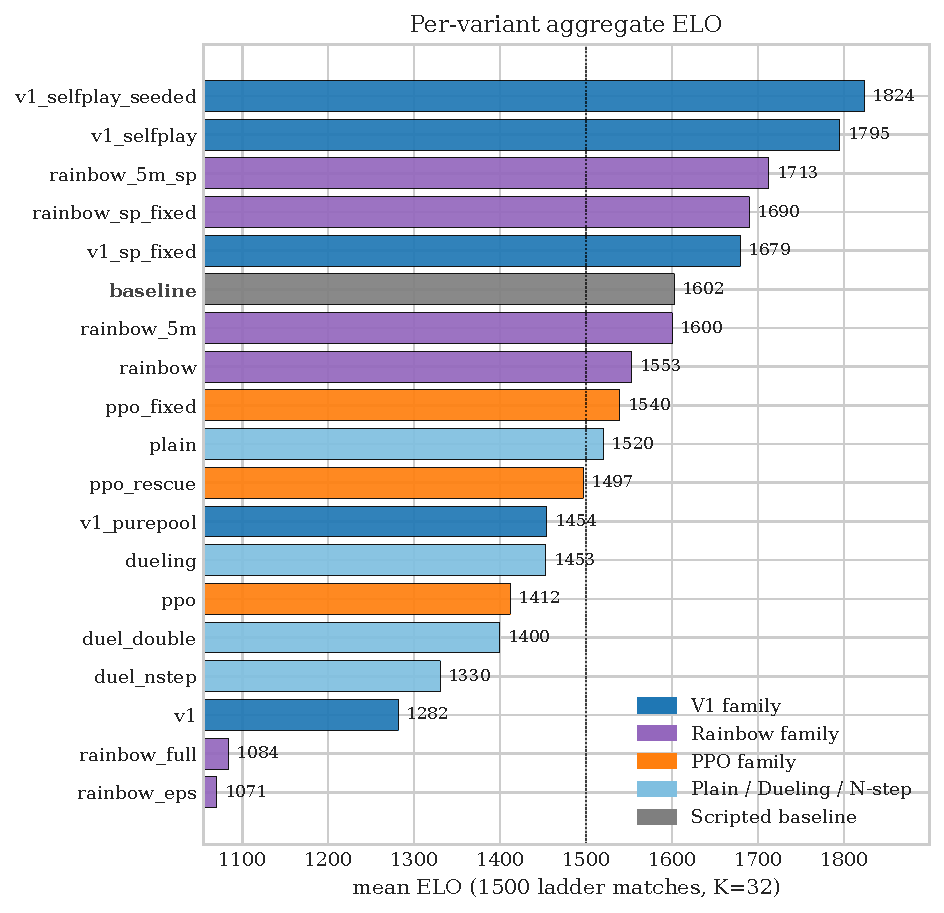
\includegraphics[width=0.82\linewidth]{figures/elo_ladder.pdf}
\vspace{-0.5em}
\caption{Round-robin Elo over 19 variants (1500 matches). Scripted
baseline (highlighted) ranks 6th; Rainbow-with-C51 variants (bottom)
collapsed (see text).}
\label{fig:elo-ladder}
\end{figure}

\textbf{Self-play vs.\ cold (same algorithm) is the largest single
gain.} \texttt{v1\_selfplay} (Elo $1795$) vs.\ \texttt{v1} cold (Elo
$1282$) is a $513$-Elo gap, $\sim$94\% expected-win.
\textbf{Full Rainbow with C51+NoisyNet collapsed:} \texttt{rainbow\_full}
($1084$) and \texttt{rainbow\_eps} ($1071$) lose 95\%+ of ladder
matches because $[v_{\min},v_{\max}]{=}[-5,+5]$ matches episode-return
extremes exactly, concentrating mass on the boundary atoms; the simpler
``Rainbow-Lite'' (Dueling+Double+$n$-step+PER) reaches Elo $1690$ on
the same budget. \textbf{\texttt{eval\_R} can disagree with Elo:}
\texttt{plain} DQN (Elo $1520$) outranks \texttt{dueling} ($1453$)
despite worse \texttt{eval\_R}, and \texttt{ppo\_fixed} (failed; Elo
$1540$) outranks \texttt{ppo\_rescue} ($1497$) despite a $+3.6$
\texttt{base\_R} advantage --- \texttt{eval\_R} measures performance
against one specific opponent, Elo against the entire ecosystem.

\paragraph{Negative results matter.} Of five hypotheses we expected to
confirm --- ``Rainbow always helps,'' ``$n$-step is a free win,''
``self-play~$>$~cold,'' ``pool quality~$>$~baseline quality,'' and
``\texttt{eval\_R} predicts Elo'' --- only \emph{self-play~$>$~cold}
survived contact with the data.
